%
%  This simple example illustrates how documents can be
%  split into smaller segments, each segment processed
%  by latex2html separately.  This document can be
%  processed through latex and latex2html with the
%  corresponding makefile.
%

\documentclass{article}         % Must use LaTeX 2e
\usepackage[plainpages=false, colorlinks=true, citecolor=black, filecolor=black, linkcolor=black, urlcolor=black]{hyperref}		
\usepackage[left=.75in,right=.75in,top=.75in,bottom=.75in]{geometry}
\usepackage{makeidx,color,boxedminipage}
\usepackage{graphicx,float}
\usepackage{amsmath,amsthm,amsfonts,amscd,amssymb} 

%%%%%%%%%%%%%%%%%%%%%%%%%%%%%%%%%%%%%%%%%%%%%%%%%%%%%%%%%%%%%%%%%%%%%%
%	Some math support.					     %
%%%%%%%%%%%%%%%%%%%%%%%%%%%%%%%%%%%%%%%%%%%%%%%%%%%%%%%%%%%%%%%%%%%%%%
%
%	Theorem environments (these need the amsthm package)
%
%% \theoremstyle{plain} %% This is the default

\newtheorem{thm}{Theorem}[section]
\newtheorem{cor}[thm]{Corollary}
\newtheorem{lem}[thm]{Lemma}
\newtheorem{prop}[thm]{Proposition}
\newtheorem{ax}{Axiom}

\theoremstyle{definition}
\newtheorem{defn}{Definition}[section]

\theoremstyle{remark}
\newtheorem{rem}{Remark}[section]
\newtheorem*{notation}{Notation}
\newtheorem*{exrcs}{Exercise}
\newtheorem*{exmple}{Example}

%\numberwithin{equation}{section}


%%%%%%%%%%%%%%%%%%%%%%%%%%%%%%%%%%%%%%%%%%%%%%%%%%%%%%%%%%%%%%%%%%%%%%
%	Macros.							     %
%%%%%%%%%%%%%%%%%%%%%%%%%%%%%%%%%%%%%%%%%%%%%%%%%%%%%%%%%%%%%%%%%%%%%%
%
%	Here some macros that are needed in this document:

\newcommand{\motion}{\mathbf{\varphi}}
\newcommand{\hmotion}{\mbox{\boldmath $\hat{\varphi}$}}
\newcommand{\cauchy}{\mbox{\boldmath $\sigma$}}
\newcommand{\eqn}[1]{(\ref{#1})}
\newcommand{\hOmega}{\hat{\Omega}}
\newcommand{\homega}{\hat{\omega}}
\newcommand{\nphalf}{n+\frac{1}{2}}
\newcommand{\nmhalf}{n-\frac{1}{2}}
\newcommand{\kmhalf}{k-\frac{1}{2}}
\newcommand{\kphalf}{k+\frac{1}{2}}
\newcommand{\picdir}{pdffig/}

\newcommand{\re}{\mathbb R}
\newcommand{\Ex}[2]{\mathcal{E}^{#2}[#1]}
%\newcommand{\log}{\text{log}[#1]}
\newcommand{\Tr}{\mathbf{Tr}}
\newcommand{\etal}{\textit{et al. }}

\newcommand{\eq}[1]{Eq.~(\ref{#1})}
\newcommand{\Fig}[1]{Fig.~\ref{#1}}

\renewcommand{\v}[1]{\ensuremath{\mathbf{#1}}}
\newcommand{\vo}[1]{\ensuremath{\boldsymbol{#1}}}
\newcommand{\pderiv}[2]{\frac{\partial #1}{\partial #2}}

\newcommand{\eps}{\boldsymbol{\epsilon}}
\newcommand{\Nu}{\boldsymbol{\nu}}
\newcommand{\Ps}{\boldsymbol{\Psi}}
\newcommand{\xii}{\boldsymbol{\xi}}
\newcommand{\Al}{\boldsymbol{\alpha}}
\newcommand{\x}{\mathbf{x}}
\newcommand{\s}{\mathbf{s}}
\newcommand{\C}{\mathbf{C}}
\newcommand{\uu}{\mathbf{u}}
\newcommand{\z}{\mathbf{z}}
\newcommand{\q}{\mathbf{q}}
\newcommand{\A}{\mathbf{A}}
\newcommand{\B}{\mathbf{B}}
\newcommand{\K}{\mathbf{K}}
\newcommand{\f}{\mathbf{f}}
\newcommand{\hc}{\mathbf{H}}
\newcommand{\R}{\mathbf{R}}
\newcommand{\G}{\mathbf{G}}
\newcommand{\y}{\mathbf{y}}
\newcommand{\Y}{\mathbf{Y}}
\newcommand{\teta}{\boldsymbol{\theta}}
\newcommand{\Teta}{\boldsymbol{\Theta}}
\newcommand{\pe}{\hat{\mathbf{p}}}
\newcommand{\pl}{\mathbf{p}^{(l)}}
\newcommand{\pt}{\mathbf{p}^\text{true}}

\newcommand{\kk}{\mathcal{K}}
\newcommand{\p}{\mathcal{P}}
%\DeclareMathOperator{\Exp}{E}
\newcommand{\V}{{\mathpzc{V}}}
\newcommand{\E}{{\mathpzc{E}}}

\newcommand{\bs}{b}
\newcommand{\bv}{\mathbf{b}}
\newcommand{\bme}{z}
\newcommand{\bvm}{\tilde{\bv}}
\newcommand{\xg}{x^G}
\newcommand{\yg}{y^G}
\newcommand{\kbf}{\mathbf{k}}
\newcommand{\mbf}{\mathbf{m}}
\newcommand{\Pbf}{\mathbf{P}}
\newcommand{\Rbf}{\mathbf{R}}
\newcommand{\Vbf}{\mathbf{V}}
\newcommand{\xbf}{\mathbf{x}}
\newcommand{\Xbf}{\mathbf{X}}
\newcommand{\Ybf}{\mathbf{Y}}
\newcommand{\zbf}{\mathbf{z}}
\newcommand{\Zbf}{\mathbf{Z}}
\newcommand{\mubf}{\boldsymbol{\mu}}
\newcommand{\nubf}{\boldsymbol{\nu}}
\newcommand{\im}{\mathrm{i}}
\newcommand{\Gammabf}{\mathbf{\Gamma}}
\newcommand{\Cbf}{\mathbf{C}}
\newcommand{\Sigmabf}{\boldsymbol{\Sigma}}
\newcommand{\zcond}{\mathbf{z}\mid\mu}
\newcommand{\zcondbf}{\mathbf{z}\mid\boldsymbol{\mu}}
\newcommand{\signalG}{\mathcal{G}\paren{\mu,\mathbf{k}}}
\newcommand{\Gscript}{\mathcal{G}}
\newcommand{\sumnn}{\sum\limits_{n=1}^N}

\newcommand{\arr}[2]{\begin{array}{#1} #2 \end{array}}
\newcommand{\lbrcarray}[2]{\left\{\arr{#1}{#2}\right.}
\newcommand{\rbrcarray}[2]{\left.\arr{#1}{#2}\right\}}
\newcommand{\argminx}{\arg\min_X}
\newcommand{\Nscript}{\mathcal{N}}

%\DeclareMathOperator{\diag}{diag} 
\newcommand{\brkarray}[2]{\bracket{\arr{#1}{#2}}}

\title{Advanced Applications of Synthetic MR and MAGiC}
\author{}
\begin{document}                % The start of the document
\maketitle

%%%%%%%%%%%%%%%%%%%%%%%%%%%%%%%%%%%%%%%%%%%%%%%%%%%%%%%%%%%%%%%%
%%%%%%%%%%%%%%%%%%%%%%%%%%%%%%%%%%%%%%%%%%%%%%%%%%%%%%%%%%%%%%%%
\section{Problem Statement}\label{sec:prob_statement}
%%%%%%%%%%%%%%%%%%%%%%%%%%%%%%%%%%%%%%%%%%%%%%%%%%%%%%%%%%%%%%%%
%%%%%%%%%%%%%%%%%%%%%%%%%%%%%%%%%%%%%%%%%%%%%%%%%%%%%%%%%%%%%%%%
Consider a magnetization signal $M_{TD}$ that is defined as
as function of 
\textbf{acquisition parameters} $\kk=\{T_R,T_D,\theta,T_E,\alpha\}$ 
and \textbf{tissue properties} $\p \equiv \{T_1,T_2,M_0\}$. 
Within the scope of this project, $T_R$=4sec, $\theta$=120\textsuperscript{o}, 
and $\alpha$=90\textsuperscript{o} are \textbf{fixed}. Delay time, $T_D$, and echo time $T_E$
are parameters under consideration for acquisition optimization. 


\begin{figure}[h] 
\centering
\begin{tabular}{ccc}
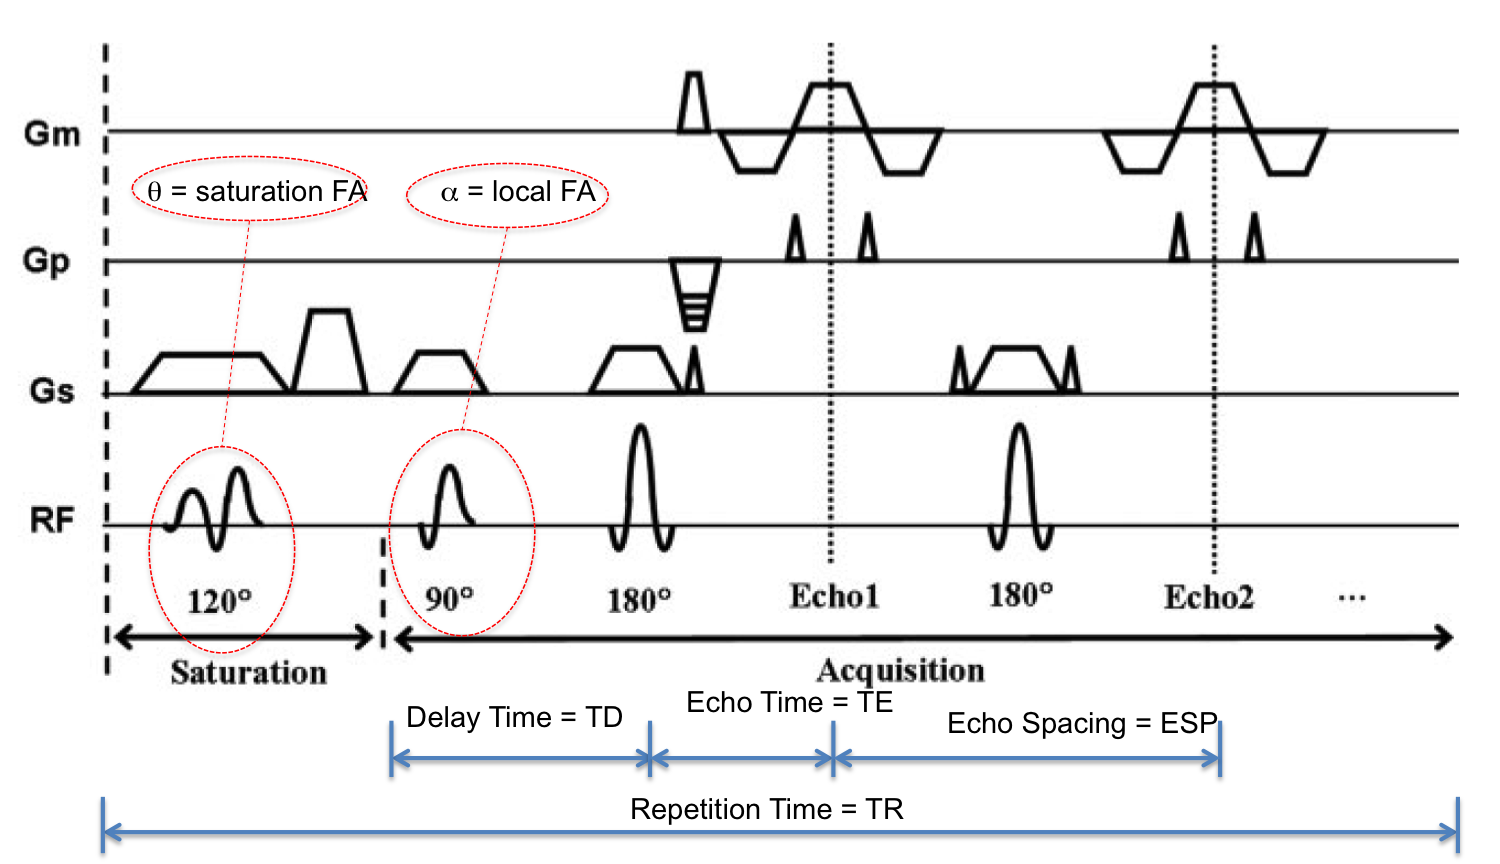
\includegraphics[width=.7\textwidth]{\picdir/PulseSequence.png} & 
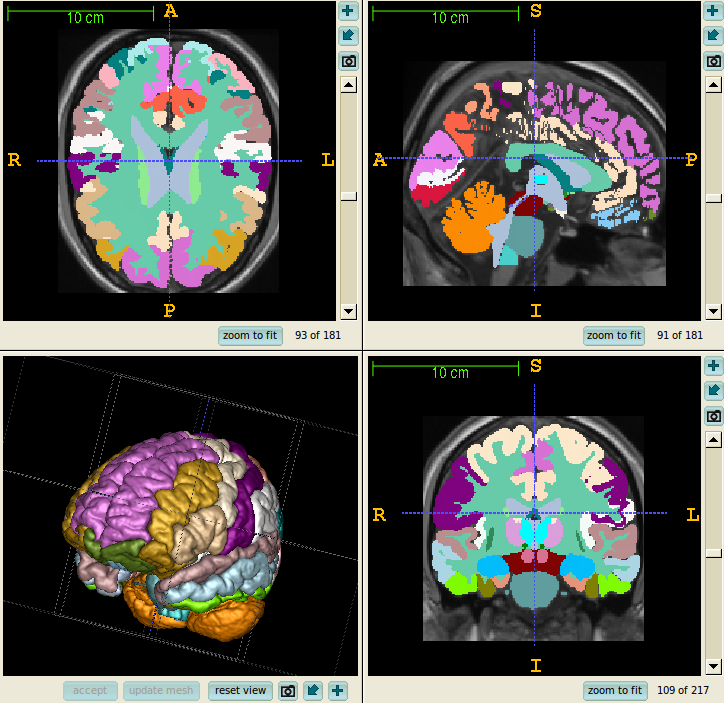
\includegraphics[width=.29\textwidth]{\picdir/NeuroBasis.png} \\
(a) & (b) \\
\end{tabular}
\caption{ 
(a) Synthetic MR Pulse sequence. (b) Neuroimaging basis.
}\label{fig:Pulsesequence}
\end{figure}

\begin{equation}\label{mtd}
M_{TD}(\kk,\p,\x)=
   M_0 e^{i\psi(\x)}
\left(
 (\x)\frac{1-(1-\cos \theta)e^{-\frac{T_D}{T_1(\x)}}-\cos \theta e^{-\frac{T_D}{T_1(\x)}}}{1-\cos \theta e^{-\frac{T_R}{T_1(\x)}}cos \alpha}
 \right) e^{-\frac{T_E}{T_2(\x)}}
\end{equation}
Here, $M_0$ is the unsaturated magnetization, $\psi(\x)$ is the measured phase offset,
$\theta$ represents the \textit{saturation} flip
angle, and $T_R$ and $T_E$ denote repetition time and echo time, respectively.
Parameters $T_1$ and $T_2$ represents relaxation times, and $\alpha$ is the
\textit{local} excitation flip angle. 
In general, excitation pulse $\alpha$ is a function of flip angle, i.e.
$\alpha=\alpha(\theta)$
{\color{red}(@kenphwang why is this?)}.
Note that the unsaturated magnetization $M_0$, along with
relaxation times $T_1$ and $T_2$, are a function of spatial coordination $\x$.
Basis functions $\phi_i$ represent the neuroanatomy. For completeness, consider
$\phi_1 = \phi_\text{gm}$,
$\phi_2 = \phi_\text{wm}$,
$\phi_3 = \phi_\text{csf}$,
$\phi_4 = \phi_\text{tumor}$ as a simplified set 
of the regions illustrated in Figure~\ref{fig:Pulsesequence}(b).
\[
T_1(\xbf)=\sum_{i=1}^{N=4} T1_i \phi_i(\xbf)
\qquad
T_2(\xbf)=\sum_{i=1}^{N=4} T2_i \phi_i(\xbf)
\qquad
M_0(\xbf)=\sum_{i=1}^{N=4} M0_i \phi_i(\xbf)
\]
	
	
\[
\bigcup_{i=1}^{N=4}\Omega_i=\Omega  \qquad  \Omega_n\cap\Omega_m=\varnothing
\qquad 
\phi_i(\xbf)=\left\{ \begin{split}
			1 & \quad x\in\Omega_i \\
			0 & \quad \text{otherwise}
                     \end{split} \right. 
\]


Assume that the signal model  for $M_{TD}$ \eqn{mtd} is our measurment model in \textbf{image space}
and is polluted with a white noise $\nu$ (with mean zero and variance $\R$). Hence, \eq{mtd} can be written as:
\begin{equation}\label{mtdobs}
z(\kk,\p)=\underbrace{M_{TD}(\kk,\p,\x)}_{h(\kk,\p)}+\nu
\end{equation}


Note that the observation $z$ is a function of control parameters $\kk$ and
parameters of interest $\p$.  The ultimate goal is to provide accurate estimate
of the parameters $\p$, given some measurements $z$. 
Precise estimation of parameters $\p$ crucially depends on the values of
control parameters $\kk=\{T_D,T_E\}$ ( $\{T_R,\theta,\alpha\}$ \textbf{fixed}).  
In other words, to ensure
performance of the estimation algorithm, one needs to select the control
parameters $\kk=\{T_D,T_E\}$ such that the observation $z$ provides
useful information about the parameters $\p$. This is achieved my maximizing
the mutual information between the measurements $z$ and parameters of interest
$\p$.  Within this framework we will consider the tissue properties to be
normally distributed Gaussian parameters.
\[
  \text{T1}_\text{WM}    =  \mathcal{N}(100ms, 20ms)  \qquad
  \text{T1}_\text{GM}    =  \mathcal{N}(120ms, 20ms)  \qquad
  \text{T1}_\text{CSF}   =  \mathcal{N}(320ms, 20ms)  \qquad
  \text{T1}_\text{Tumor} =  \mathcal{N}(300ms, 20ms)
\]
\[
  \text{T2}_\text{WM}    =  \mathcal{N}(100ms, 20ms)  \qquad
  \text{T2}_\text{GM}    =  \mathcal{N}(120ms, 20ms)  \qquad
  \text{T2}_\text{CSF}   =  \mathcal{N}(320ms, 20ms)  \qquad
  \text{T2}_\text{Tumor} =  \mathcal{N}(300ms, 20ms)
\]
\[
  \text{M0}_\text{WM}    =  \mathcal{N}(100??, 20??)  \qquad
  \text{M0}_\text{GM}    =  \mathcal{N}(120??, 20??)  \qquad
  \text{M0}_\text{CSF}   =  \mathcal{N}(320??, 20??)  \qquad
  \text{M0}_\text{Tumor} =  \mathcal{N}(300??, 20??)
\]
{\color{red}(@kenphwang need exact numbers)}


%%%%%%%%%%%%%%%%%%%%%%%%%%%%%%%%%%%%%%%%%%%%%%%%%%%%%%%%%%%%%%%%
%%%%%%%%%%%%%%%%%%%%%%%%%%%%%%%%%%%%%%%%%%%%%%%%%%%%%%%%%%%%%%%%
\section{Optimal ($T_D$,$T_E$) Design}\label{oed}
%%%%%%%%%%%%%%%%%%%%%%%%%%%%%%%%%%%%%%%%%%%%%%%%%%%%%%%%%%%%%%%%
%%%%%%%%%%%%%%%%%%%%%%%%%%%%%%%%%%%%%%%%%%%%%%%%%%%%%%%%%%%%%%%%
As discussed before, performance of estimation process crucially depends on the value of control parameters $\kk$. Hence, it is important to develop mathematical tools to identify the control parameters $\kk$ such that they provide the best observation data for accurate estimation of parameter $\p$. This is equivalent with maximizing the mutual information between the observation data and parameters $\p$. Based on information theory, mutual information is defined as the reduction of uncertainty in one parameter due to knowledge of the other parameter.

\begin{equation} \label{mi}
I(\p;z)=\int_z\int_p p(\p,z)\ln\left(\frac{p(\p,z)}{p(\p)p(z)}\right)d\p dz
\end{equation}

We make use of Bayes theorem to simplify the above equation. By substituting $p(\p,z)$ with $p(z|\p)p(\p)$, \eq{mi} can be written as:

\begin{equation} \label{mi2}
I(\p;z)=\int_z\int_p p(z|\p)p(\p)\ln\left(\frac{p(z|\p)p(\p)}{p(\p)p(z)}\right)d\p dz
\end{equation}
Or,
\begin{equation} \label{mi3}
I(\p;z)=\int_z\int_p p(z|\p)p(\p)\ln\left[p(z|\p)\right]d\p dz - \int_z p(z) \ln p(z)dz
\end{equation}



Note that due to dependence of observation data $z$ on control parameters, the mutual information $I(\p;z)$ is a function of control parameter $\kk$. In order to maximize the reduction of uncertainty in parameter estimate (i.e. to have the most confident estimates of the parameter $\p$), one can simply maximize the mutual information between the observation data and parameters of interest:

\begin{equation}\label{mimax}
\max_{\kk} I(\p;z)
\end{equation}

The above maximization results in \textit{optimal} values of control parameter $\kk$ for accurate estimation of parameter $\p$. Note that in \eq{mi3}, $p(z|\p)$ is defined as a Gaussian distribution with mean $h(\kk,\p)$ and variance $\R$. As well, $p(\p)$ denotes the prior distribution of parameter $\p$, which for the ease of calculations, is considered to be a Gaussian distribution with some prior mean $\hat{\p}^-$ and prior covariance $\Sigma^-$, i.e. $p(\p)\sim \mathcal{N}(\hat{p}^-,\Sigma^-)$. Method of quadrature points can be used to evaluate \eq{mi3}. 

We emphasize here that the mutual information will be the same on different pixels with the same tissue types. This is due to the similarities in statistics of $\p$ between the two different pixels with the same tissue properties. In other words, whenever two different pixels have the same tissue properties, then the distribution of parameter $\p$, denoted by $p(\p)$, is the same and so is the value of mutual information. Hence, there is no need to evaluate the mutual information for each pixel in a region with the same tissue type. 

On the other hand, in a case that the tissue properties for each pixel are different from the other, then the mutual information needs to be evaluated for each and every pixel of interest.

The final plot over delay time and echo time is shown in Figure~\ref{fig:MIMapTDTE}.
The current acquistion utilizes 8 total combinations of (effective) echo times 
and delay times, 2 echo times and 4 delay times.

The information content of this acquisition scheme is calculated as the superposition
\[
 I^\text{current} = \sum_{i=1}^8 I((T_D, T_E)_i)
\qquad \text{\color{red}(@kenphwang need exact numbers)}
\]
\[
   \left(T_D, T_E\right) = 
   \left\{
   \text{(20ms, 15ms),(40ms, 15ms),(70ms, 15ms),(90ms, 15ms),
         (20ms, 35ms),(40ms, 35ms),(70ms, 35ms),(90ms, 35ms)}
   \right\}
\]
An optimal acquisition strategy either maintains or improves this information content with
less samples to (1) improve time and (2) accuracy.
\[
  I^\text{current} < I^\text{optimal} = \sum_{i=1}^{M \leq 8} I((T^*_D, T^*_E)_i)
\]

\begin{figure}[h] 
\centering
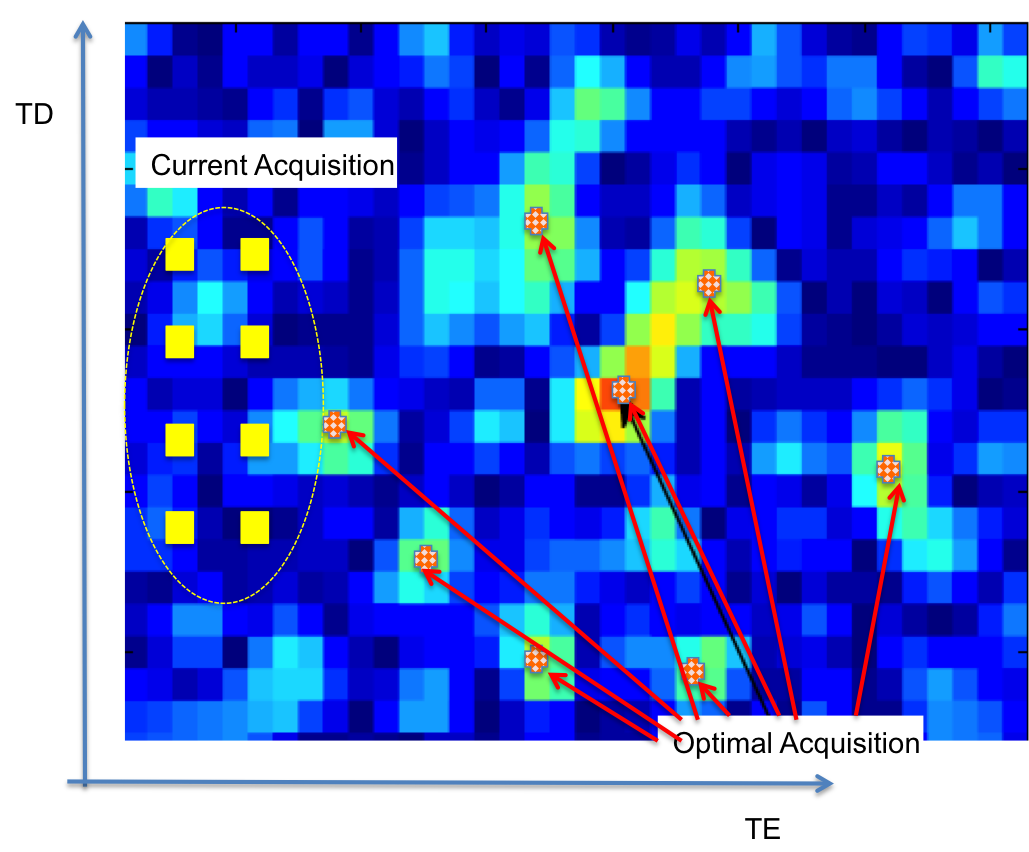
\includegraphics[width=.7\textwidth]{\picdir/MIMapTDTE.png} 
\caption{ 
Information content as function of $(T_D, T_E)$
}\label{fig:MIMapTDTE}
\end{figure}

%%%%%%%%%%%%%%%%%%%%%%%%%%%%%%%%%%%%%%%%%%%%%%%%%%%%%%%%%%%%%%%%
\subsection{MI Approximations}
%%%%%%%%%%%%%%%%%%%%%%%%%%%%%%%%%%%%%%%%%%%%%%%%%%%%%%%%%%%%%%%%

{\color{red}(@dmitchell412 need Variance calculation algorithm compiled here with Quadrature)}

(Copy approximation from @madankan paper)

\[
 MI = H(z) \approx \Sigma_z = 
\]

As mentioned earlier, one of the main challenges in MRI technique is to effectively determine the optimal locations on $k-$space such that they provide the best estimate for the image. In other words, we are looking for the measurement data such that they provide the most confident estimates of uncertain parameters. This is equivalent with finding the measurement data that result in most reduction of uncertainty in parameter estimates. Based on the Information Theory \cite{cover2012elements}, the reduction of uncertainty in one parameter due to the knowledge of the other variable is known as \textit{Mutual Information}. Hence, a good measurement data is the one that provides us the maximum amount of mutual information. Information theoretic approaches and the concept of mutual information has been used in numerous works for optimal sensor placement and sensor management \cite{bourgault2002information,martinez2006optimal,tharmarasa2007large,williams2007approximate,krause2008,choi2010continuous,julian2012distributed,madankan_jae,Madankan_dydess}. The concept of mutual information is also recently being used for optimal measurement design in functional MRI (fMRI) \cite{yan2014linear}. In the following, we first describe the concept of mutual information. Then the mathematical details for finding the optimal locations on $k-$space are presented.

\subsubsection*{Mutual Information as a Measure of Sensor Performance}
According to information theory, the mutual information \cite{cover2012elements} between the model forecast $\mathcal{U}$ and measurement $z$ can be written as

\begin{equation}\label{mutual_info_u}
I(\mathcal{U}(\mu,\bar{k});z) = \int_{z}\int_{\mathcal{U}} p(\mathcal{U},z)\ln\left(\frac{p(\mathcal{U},z)}{p(\mathcal{U})p(z)}\right)d\mathcal{U} dz
\end{equation}

Since the uncertain parameter $\mu$ is the only source of uncertainty in model forecast $\mathcal{U}$, one can evaluate the mutual information between the uncertain parameter $\mu$ and measurement $z$, instead of \eq{mutual_info_u}:

\begin{equation}\label{mutual_info}
%I(k^\mu;z^k) \equiv 
I(\mu;z) = \int_{z}\int_{\mu} p(\mu,z)\ln\left(\frac{p(\mu,z)}{p(\mu)p(z)}\right)d\mu dz
\end{equation}
Using Bayes' rule, $p(\mu,z)$ can be written as

\[p(\mu,z)=p(\mu|z)p(z)\]
Hence $I(\mu;z)$ will be equal to:
\begin{eqnarray}\label{info}
I(\mu;z) = \int_{z} \underbrace{\int_{\mu} p(\mu|z)ln\left(\frac{p(\mu|z)p(z)}{p(\mu)p(z)}\right)d\mu}_{D_{KL}(p(\mu|z))||p(\mu)} p(z) dz
\end{eqnarray}
or,
\begin{equation}
I(\mu;z)=\mathcal{E}_z[D_{KL}\left(p(\mu|z))||p(\mu)\right)]
\end{equation}
  
where, $D_{KL}\left(p(a)||p(b)\right)$ denotes the KL distance between two probability density functions $p(a)$  and $p(b)$. Hence, mutual information can be interpreted as the average Kullback-Leiber distance between the prior pdf $p(\mu)$ and the posterior pdf $p(\mu|z)$. By maximizing the mutual information, one inherently maximizes the difference between the prior and posterior distributions of the parameter $\mu$, thus leading to a better measurement and estimate.


\subsection{Optimal Locations on k-space}\label{subsec:kspace}
Note that due to dependence of observation data $z$ on $k-$space parameters, the mutual information $I(\mu;z)$ is also a function of $(k_x,k_y,k_z)$ parameters. Hence, our goal is to look for a set of optimal locations $(k_x^j,k_y^j,k_z^j),\ j=1,2,\cdots,N$ such that they maximize the mutual information. This can be mathematically described as the following optimization problem:

\begin{equation}\label{cost1}
\max_K J(K) = \max_{K} I(\mu;\mathbf{z})
\end{equation}
where, $K=\{(k_x^1,k_y^1,k_z^1),\cdots,(k_x^N,k_y^N,k_z^N)\}$ denotes the coordinates of $N$ observations on $k-$space and $\mathbf{z}=\{z_1,z_2,\cdots,z_N\}$ is the set of all $N$ observations in hand. 

Note that obtained $k$-space points are completely independent from \textit{noise realizations}, while \textit{statistics of the noise} will affect the location of k-space points. For instance, if the standard deviation of noise increases, it will result in a less confident estimate of parameter $\mu$, and vice versa. In extreme case, when standard deviation of noise goes to infinity, i.e. when SNR approaches to zero, there would not be any useful information in k-space measurements and proposed algorithm returns the same prior estimates of $\mu$. On the other hand, when SNR goes to infinity (i.e. standard deviation of noise goes to zero), the proposed algorithm will be much more confident about the parameter estimate $\mu$ and correspondingly temperature estimate. 
%Unfortunately, solving the above optimization problem is computationally intractable for most of the practical applications. Hence, one needs to simplify the original optimization problem and find the approximate solution for optimal location of each observation. \textit{Assuming} measurement data to be statistically independent from each other, one can use heuristic problem solving techniques like greedy algorithm \cite{bertsekas_book} to simplify the aforementioned optimization. Using the greedy algorithm, original optimization problem can be simplified to:
%Note that due to independence of measurement data, one can rewrite \eq{cost1} as:

%\begin{equation}\label{cost2}
%\max_K J(K)=\max_{K} \sum\limits_{j=1}^{N} I(\mu;z_j)
%\end{equation}
%and since the mutual information $I(\mu;z_j)$ is a scalar positive quantity, \eq{cost2} can be written as the following:
%
%\begin{align}
%\max_K J(K)=& \sum\limits_{j=1}^{N}\max_{(k_x^j,k_y^j,k_z^j)} I(\mu;z_j)\label{cost3}\\
%\text{subject to: } & \nonumber\\
%&(k_x^i,k_y^i,k_z^i) \neq (k_x^j,k_y^j,k_z^j) \label{cons}
%\end{align}
%where, \eq{cons} is considered to avoid the redundancy in observations. Intuitively, \eq{cost3} tries to find the optimal locations for each observation on $k-$space such that it maximizes the mutual information between the measurement and uncertain parameter $\mu$.


\subsection{A Simpler Alternative: Maximizing the Variance}\label{susec:variance}
Unfortunately, evaluation of mutual information and solving the above optimization problem is computationally intractable for most of the practical applications. Hence, one needs to simplify the original optimization problem and find the approximate solution for optimal location of each observation. A simpler alternative in finding useful $k-$space locations is to maximize the entropy (uncertainty) in model outputs $\mathcal{U}$, instead of maximizing the mutual information $I(\mu;z)$ \cite{krause2008}. Based on information theory, the entropy of $\mathcal{U}$, denoted by $h(\mathcal{U})$ is defined as:
%As we discussed in section \ref{sec:dyn_data}, mutual information can be expressed as the reduction of uncertainty (entropy), i.e. $I(\mathcal{U},z)$ can be expressed as
%
%\begin{equation}\label{mutualinfo_entropy}
%I(\mathcal{U},z)=h(\mathcal{U})-h(\mathcal{U}|z)
%\end{equation}
%where, $h(\mathcal{U})$ denotes the entropy of $\mathcal{U}$, and is defined as

\begin{equation}\label{entropy}
h(\mathcal{U})=-\int_{\mathcal{U}} ln\left(p(\mathcal{U})\right)p(\mathcal{U})d\mathcal{U}
\end{equation}
where, $p(\mathcal{U})$ is the probability density function of $\mathcal{U}$. % As well, $h(\mathcal{U}|z)$ represents the entropy of $\mathcal{U}$, given the measurement $z$.
%Now, according to \eq{mutualinfo_entropy}, one can write
%\begin{equation}\label{info_entro_max}
%\max I(\mathcal{U},z)=\max \left\lbrace h(\mathcal{U})-h(\mathcal{U}|z)\right\rbrace
%\end{equation}
%or
%\begin{equation}\label{info_entro_max}
%\max I(\mathcal{U},z) \geq \max h(\mathcal{U}) - \max h(\mathcal{U}|z)
%\end{equation}
%Looking at \eq{info_entro_max}, one can see that maximizing the entropy $h(\mathcal{U})$ maximizes the lower bound of $I(\mathcal{U},z)$. 
One can simplify the problem by just maximizing the entropy of model outputs, instead of maximizing the mutual information. We emphasize here that this simplification may have its drawback in not giving the \textit{globally} optimal locations on $k-$space, but as we will show in the following, it will result in great simplification of the problem. 

To proceed with maximizing the entropy $h(\mathcal{U})$, we first note that based on Maximum Entropy Principle \cite{cover2012elements}, probability density function $p(\mathcal{U})$ can be parametrized in terms of its central moments as

\begin{equation}\label{pu_entropy}
p(\mathcal{U})=\lim_{N\rightarrow \infty} \left(e^{\sum\limits_{n=0}^N \lambda_n (\mathcal{U}-\hat{\mathcal{U}})^n}\right),\quad \lambda_n \in \re
\end{equation}

where, $\hat{\mathcal{U}}$ is provided by \eqref{expx1U}. By substituting \eq{pu_entropy} in \eq{entropy}, we will have:
$  $
\begin{align}
h(\mathcal{U})=-\int_{\mathcal{U}} \lim_{N\rightarrow \infty} \left(\sum\limits_{n=0}^\infty \lambda_n (\mathcal{U}-\hat{\mathcal{U}})^n\right) p(\mathcal{U})d(\mathcal{U})\nonumber\\
= \lim_{N \rightarrow \infty} (-\lambda_0 - \sum\limits_{n=2}^{N} \lambda_n m_n) \label{entropy_moments}
\end{align}
where, $m_n$s are the central moments of $\mathcal{U}$, defined by \eq{expx1_ctrU}. Hence, entropy of $p(\mathcal{U})$ can be described in terms of its central moments, as shown in \eq{entropy_moments}. Now, by approximating $p(\mathcal{U})$ with its first two moments and truncating the above expansion (i.e. letting $N=2$), we have 

\begin{equation}\label{entropy_var}
h(\mathcal{U})\simeq -\lambda_0-\lambda_2 m_2,\quad \lambda_0,\lambda_2 \in \re
\end{equation}
Therefore, to maximize the entropy one can only maximize the variance, i.e.
\begin{eqnarray}\label{entropy_var_max}
\max_{K} h(\mathcal{U})= -\lambda_0 -\lambda_2 \max_{K}(m_2), \quad \lambda_0,\lambda_2 \in \re
\end{eqnarray}
\textcolor{black}{subject to:
\begin{equation}\label{sparsity_con}
|K^i-K^j|\geq N_d,\quad \forall\ i,j\in 1,2,\cdots,N,\quad i\neq j 
\end{equation}}
where, $|K^i-K^j|=|(k_x^i,k_y^i,k_z^i)-(k_x^j,k_y^j,k_z^j)|$ denotes the distance between the $i^{th}$ and $j^{th}$ locations on $k-$space and $m_2=Var(\mathcal{U})$ is defined from \eq{expx1_ctrU}. Hence, the locations on $k-$space with the highest value of variance for $\mathcal{U}$ are a good approximation of optimal locations for data observations. 

\textcolor{black}{\eq{sparsity_con} is considered to ensure that every distinct pair of $k-$space observations are at least by a distance $N_d$ apart from each other. This constraint is used in order to compensate possible dependencies that can be introduced due to approximation of the original problem. We assumed $N_d=1$ through this manuscript.}

\textcolor{black}{One should note that different order of truncation (i.e. different values of $N$) can be used to approximate the entropy in \eq{entropy_moments}. Clearly, higher order approximation (greater values of $N$) leads to more accurate approximation of entropy. However, the downside of using higher order terms is that one needs to find the corresponding $\lambda_n$ coefficients for each term. Finding corresponding $\lambda_n$ coefficients requires solving an optimization problem which could increase computational cost of the whole procedure. Hence, lower order approximation of entropy is of more interest due to real time applications of the proposed technique.}

%As explained in section \ref{subsec:kspace}, solution of associated optimization problem with maximizing mutual information can be computationally intractable in presence of large number of measurements. In addition, evaluation of mutual information $I(\mu;z)$ can be computationally expensive due to associated integrations in \eq{mutual_info}. A simpler alternative to avoid these complexities is to find the locations on $k-$space which posses the highest variability in model predictions. To achieve this, one first needs to perform non-uniform Fourier transform on the Pennes bioheat model outputs using \eq{ymodel} and then, variance of model predictions can be  calculated as given in \eq{expx1_ctrU}, i.e.
%
%\begin{equation}\label{varkspace}
%Var(\mathcal{U})=\sum_{q=1}^{M} w_q(\mathcal{U}(\x,\mu(\xii^q),t)-\hat{\mathcal{U}})^2
%\end{equation}
%where, $\hat{\mathcal{U}}$ is the expected value of $\mathcal{U}$, calculated using \eq{expx1U}. Now, the locations on $k-$space with highest value of the variance are the \textit{most useful} locations for data observations. 
The intuition behind the idea of maximizing the variance is that the points on $k-$space with lower value of variance are less sensitive to model perturbations (resulted from parameter uncertainties) and vice versa. Hence, it is better to select the points on $k-$space with highest sensitivity with respect to model uncertainties. For instance, a point with zero variance on $k-$space will not be a good candidate for data observation since no matter what the values of uncertain parameters are, model output will always be the same at that specific point. On the other hand, a point on $k-$space with large value of variance means that the model output at that location is \textit{highly sensitive} to model uncertainties. Hence, a measurement at that $k-$space location would be of more interest. Therefore, the points with highest values of variance of $\mathcal{U}$ are \textit{better candidates} for data observations. 

%Note that against the mutual information, calcuation of variance of model outputs is very simple and computationally affordable. In addition, solving the optimization problem associated with finding the points with highest values of variance is a much simpler task, comparing with solution of \eq{cost3}.


\subsection{Adaptation to Practical $k-$space Sampling}\label{susec:var_kspace}
It is well known that practically, $k-$space sampling occurs along readout lines, rather than just sparse points on $k-$space. Hence, one needs to modify the idea of variance maximization in order to make it applicable to practical $k-$space sampling. To do so, we propose to perform the $k-$space sampling along the readout lines which their points posses the higher value of variance, i.e.

\begin{equation}\label{var2d}
\max_{K_y} \sum_{k_x=1}^{N_x} m_2(k_x,k_y)
\end{equation}
where, $K_y=\{k_y^1,\cdots,k_y^N\}$ and $N_x$ denotes the total number of points along the $k_x$ axis on $k-$space. Similarly, in $3-$dimensional $k-$space sampling, one can write
\begin{equation}\label{var3d}
\max_{K_{xy}} \sum_{k_z=1}^{N_z} m_2(k_x,k_y,k_z)
\end{equation}
where, $K_{xy}=\{(k_x^1,k_y^1),\cdots,(k_x^N,k_y^N)\}$ and $N_z$ denotes the total number of points along the $k_z$ axis on $k-$space. 

The major benefit of using \eq{var2d} and \eq{var3d} instead of maximizing \eq{entropy_var_max} is that it provides a more practical scheme for optimal $k-$space undersampling by providing the most informative readout lines, rather than the most informative points. In addition, less computational effort is required to solve  \eq{var2d} and \eq{var3d} comparing to \eq{entropy_var_max}. Note that after finding the optimal readout lines through maximizing \eq{var2d} and \eq{var3d} all the points along those readout lines are used for model - data fusion.



%%%%%%%%%%%%%%%%%%%%%%%%%%%%%%%%%%%%%%%%%%%%%%%%%%%%%%%%%%%%%%%%
\subsection{MI Calculations}
%%%%%%%%%%%%%%%%%%%%%%%%%%%%%%%%%%%%%%%%%%%%%%%%%%%%%%%%%%%%%%%%

{\color{red}(@dmitchell412 need Entropy calculation algorithm compiled here using
linearization about quadrature points)}

A more direct calculation of the entropy is given as
\[
 MI = H(z) \approx 
\]

\begin{figure}[h] 
\centering
\begin{tabular}{ccc}
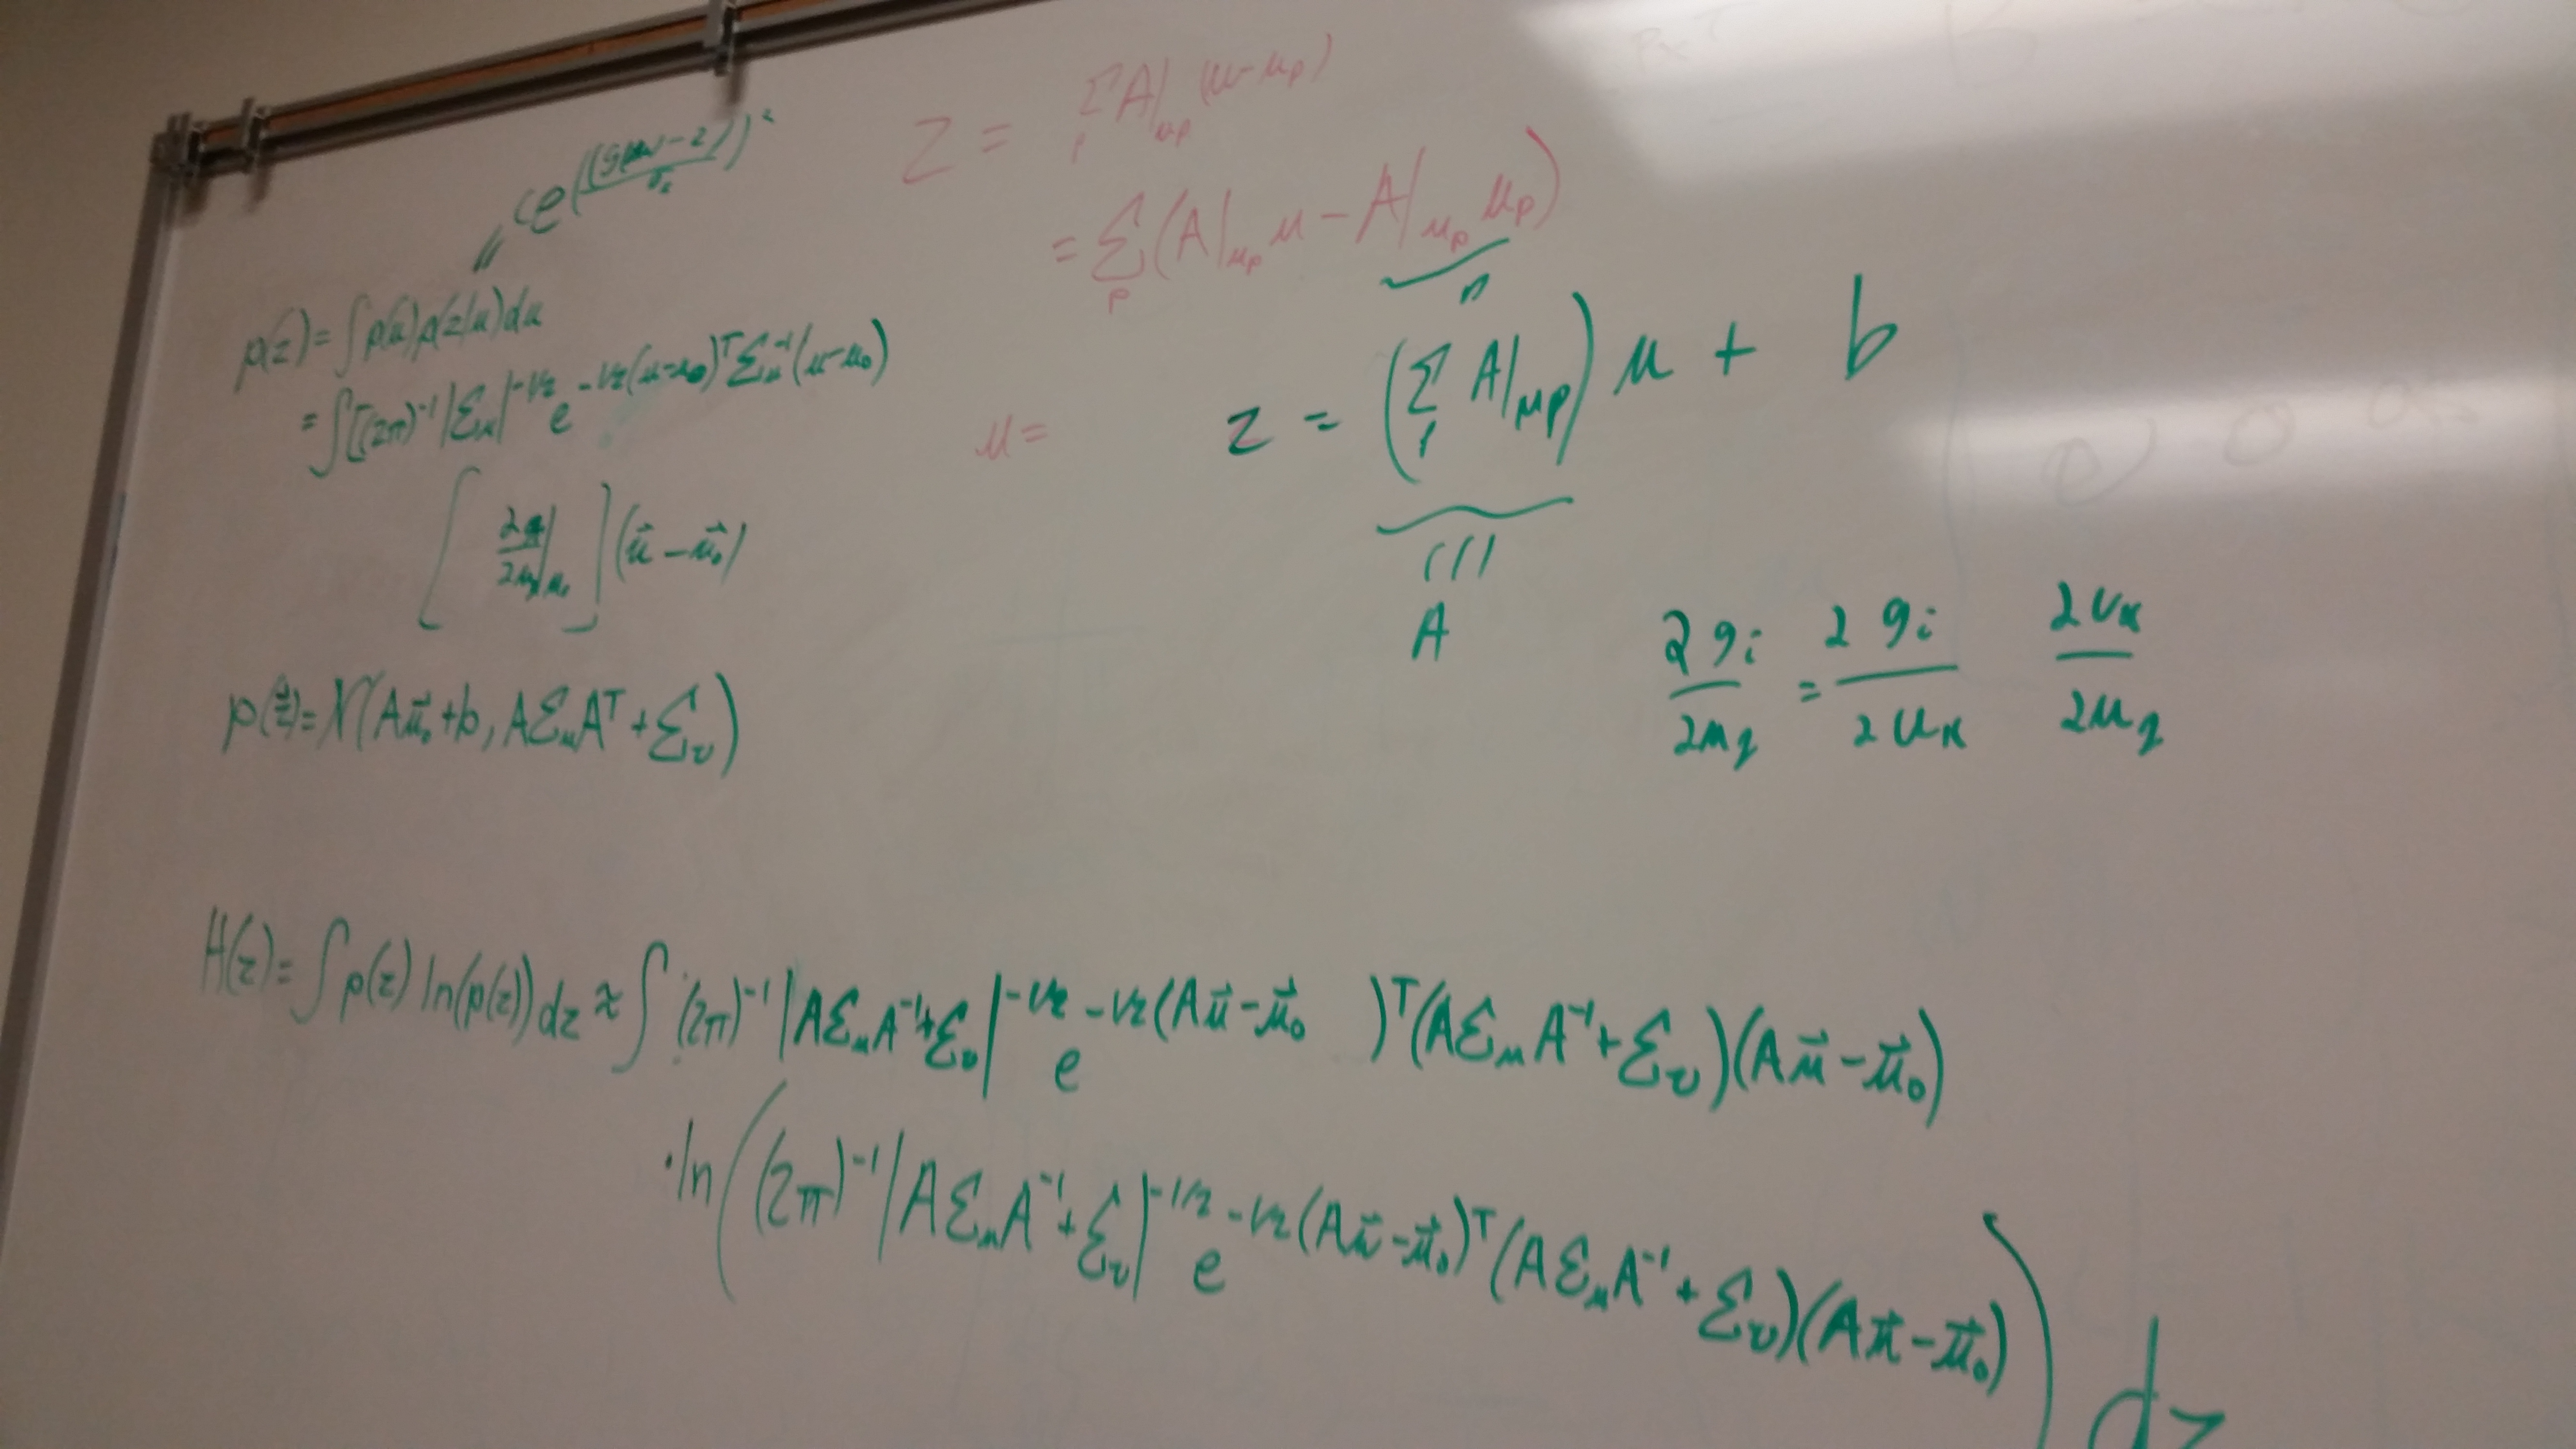
\includegraphics[width=.5\textwidth]{\picdir/20160519_115937.jpg} & 
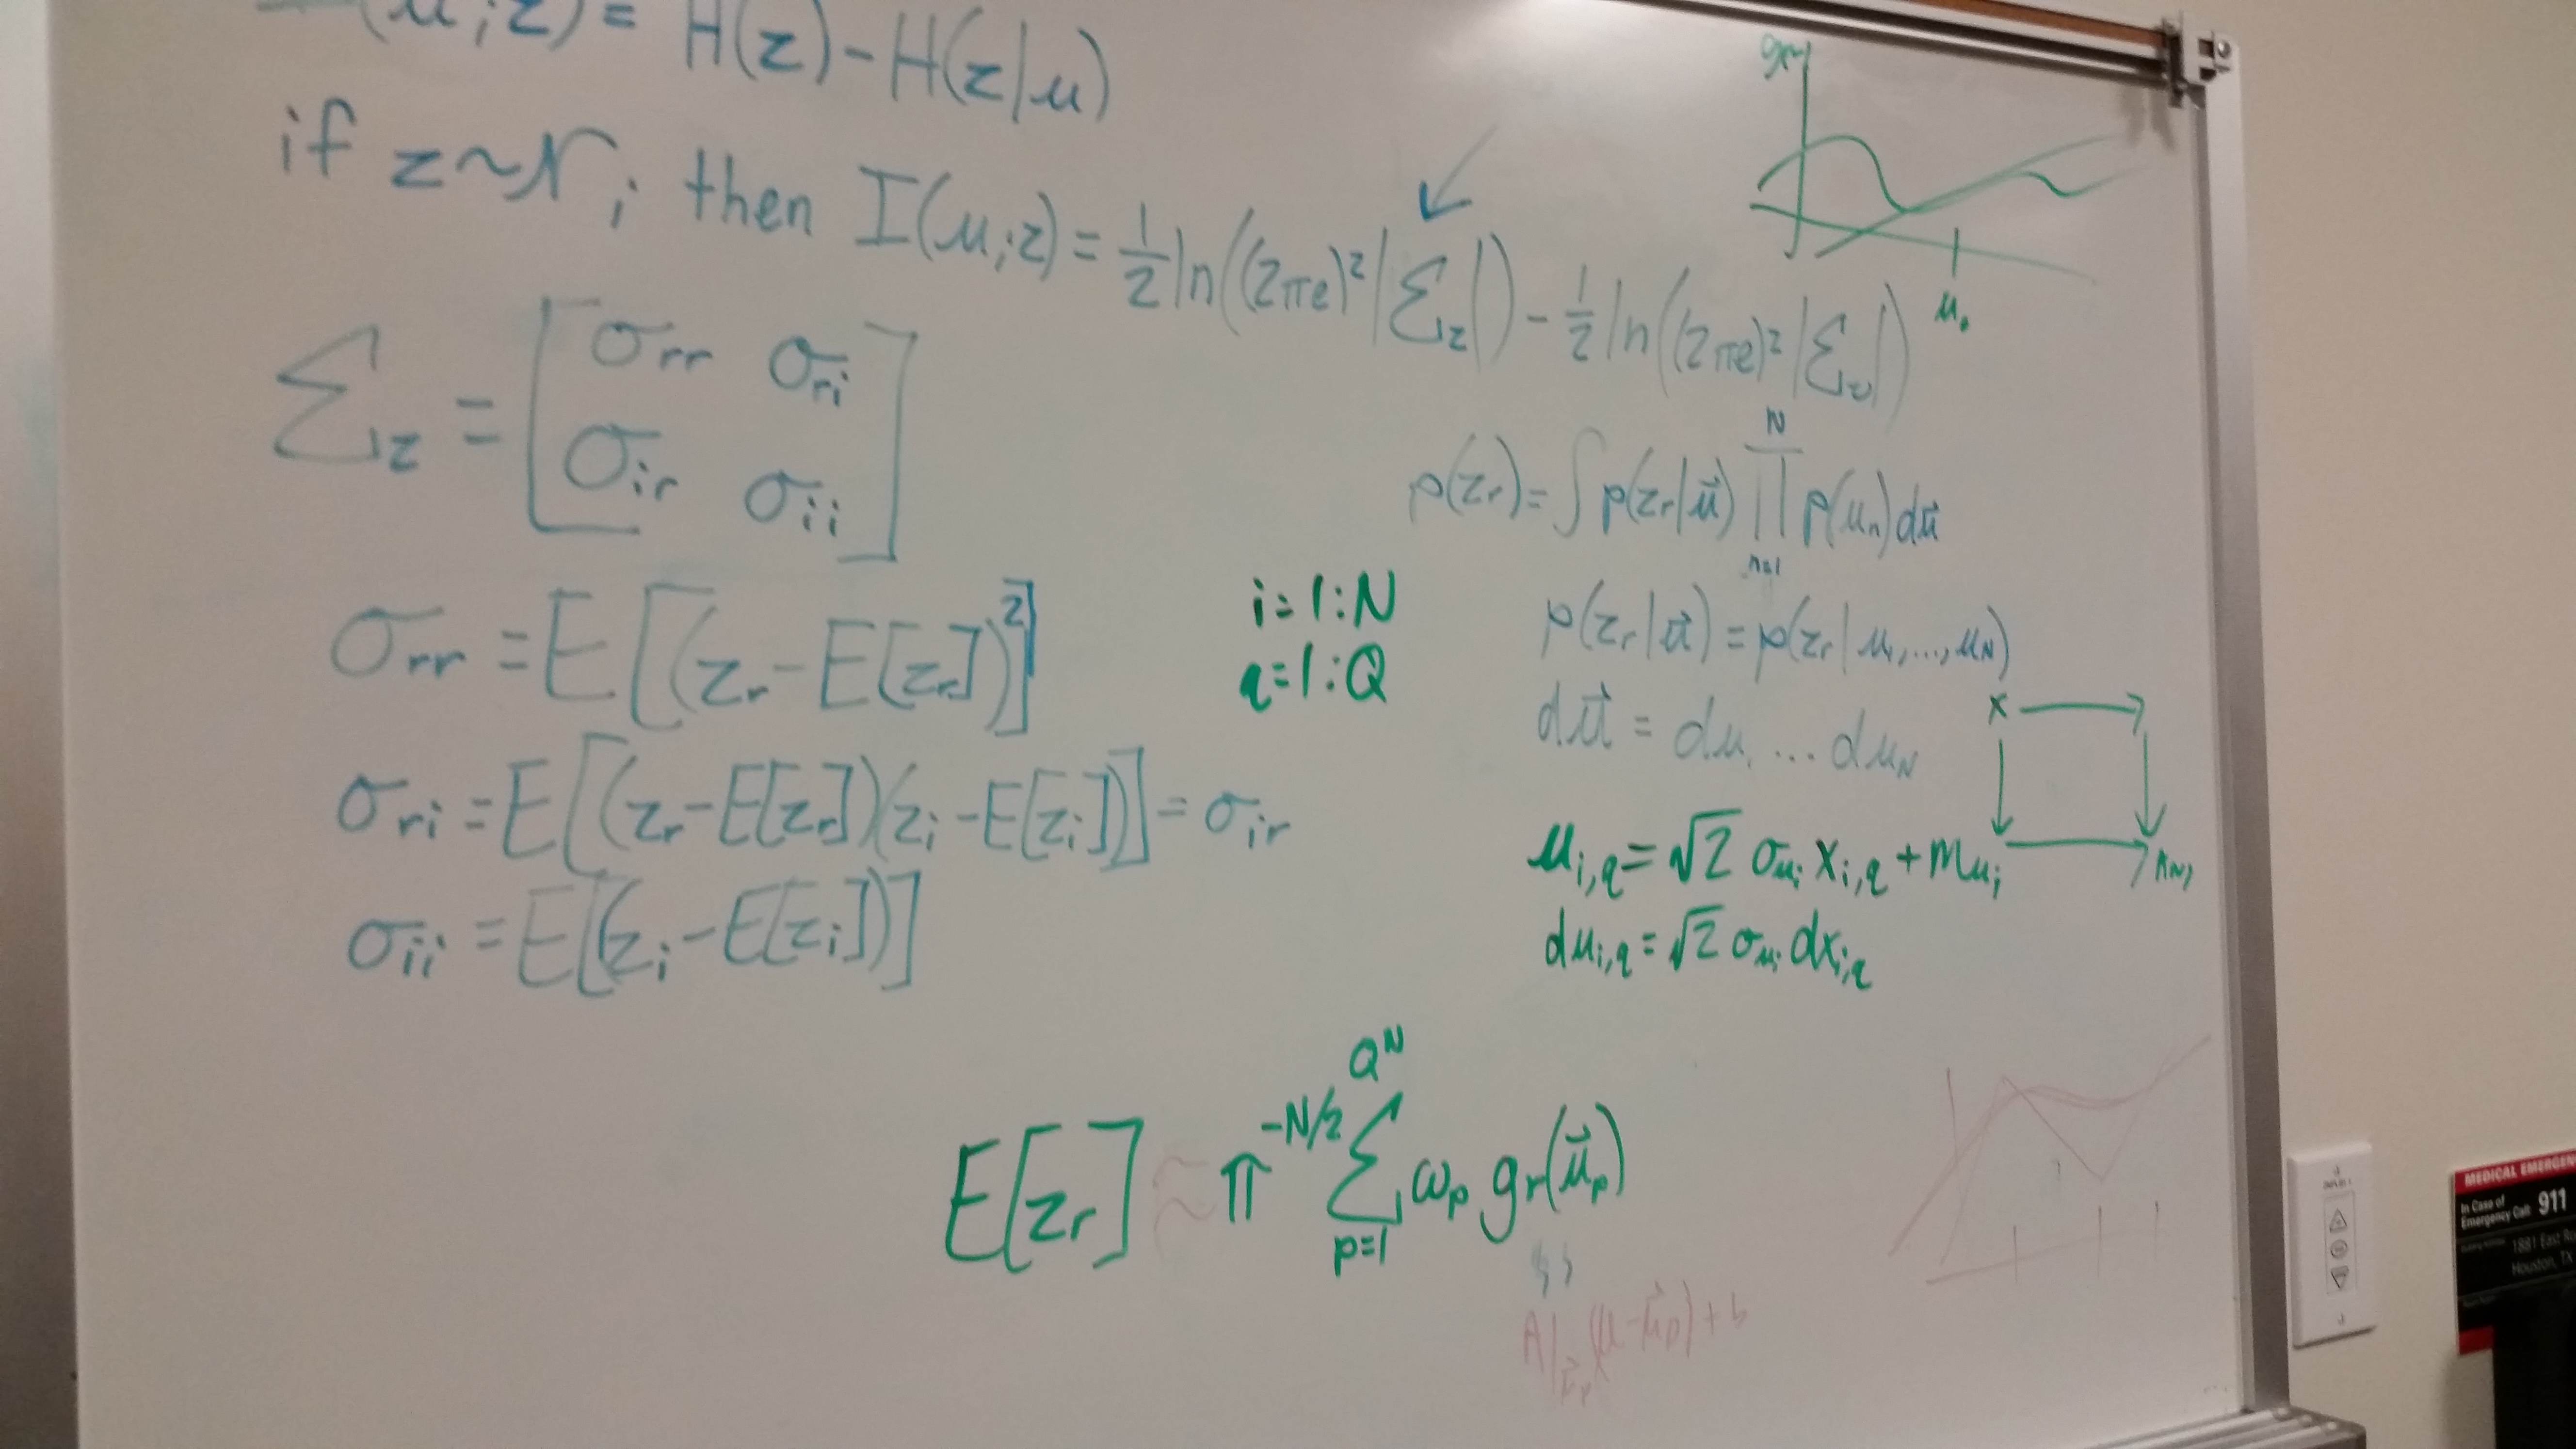
\includegraphics[width=.49\textwidth]{\picdir/20160519_115947.jpg} \\
\end{tabular}
\caption{ 
\color{red}
WIP - @dmitchell412 Need higher order entropy approximation
}\label{fig:Pulsesequence}
\end{figure}

%%%%%%%%%%%%%%%%%%%%%%%%%%%%%%%%%%%%%%%%%%%%%%%%%%%%%%%%%%%%%%%%
\section{WIP - Model Data Fusion}\label{da}
%%%%%%%%%%%%%%%%%%%%%%%%%%%%%%%%%%%%%%%%%%%%%%%%%%%%%%%%%%%%%%%%
%%%%%%%%%%%%%%%%%%%%%%%%%%%%%%%%%%%%%%%%%%%%%%%%%%%%%%%%%%%%%%%%
After finding the optimal values of the control parameter $\kk$, we can proceed and perform the model-data fusion to get a better understanding about the uncertainties involved in parameters $\p$.
The fusion of observational data with mathematical model predictions promises to provide greater understanding of physical phenomenon than either approach alone can achieve. In here, a minimum variance framework is being used for model - data fusion. Based on minimum variance technique, posterior statistics of parameter $\p$ can be written as:

\begin{eqnarray}
\hat{\p}^+=\hat{\p}^-+\K[z-\underbrace{\Ex{h(\kk,\p)}{-}}_{h^-}]\label{minvarmean}\\
\Sigma^+=\Sigma^-+\K\Sigma_{hh}\K^T\label{minvarvar}
\end{eqnarray}
where, %$z\equiv \tilde{M}_{TD}$ and 
the gain matrix $K$ is given by
\begin{eqnarray}\label{kgain}
\K=\Sigma_{\p z}\left(\Sigma_{hh}^-+\R\right)^{-1}
\end{eqnarray}

Here, $\hat{\p}^-$ and $\hat{p}^+$ represent prior and posterior values of the mean for parameter vector $\p$, respectively:
\begin{eqnarray}
\hat{\p}^-\equiv \Ex{\p}{-}=\int \p^- p(\p)d\p \label{Pprior}
\hat{\p}^+\equiv \Ex{\p}{+}=\int \p^+ p(\p)d\p \label{Pposterior}
\end{eqnarray}
where, $p(\p)$ denotes the probability density function of parameter $\p$. Similarly, the prior and posterior covariance matrices $\Sigma^{-}$ and $\sigma^+$ can be written as:

\begin{eqnarray}
\Sigma^-\equiv\Ex{(\p-\hat{\p}^-)(\p-\hat{\p}^-)^T}{}\\
\Sigma^+\equiv\Ex{(\p-\hat{\p}^+)(\p-\hat{\p}^+)^T}{}
\end{eqnarray}

The matrices $\Sigma_{\p z}$ amd $\Sigma_{hh}$ are defined as:

\begin{eqnarray}
\Sigma_{\p z} \equiv\Ex{(\p-\hat{\p})(h-\hat{h}^-)^T}{}\\
\Sigma_{hh} \equiv\Ex{(h-\hat{h}^-)(h-\hat{h}^-)^T}{}
\end{eqnarray}

\eq{minvarmean} along with \eq{minvarvar} provide posterior mean and covariance of parameter $\p$ given observation data $\tilde{z}$ and model predictions $h(\kk,\p)$.
We emphasize here that the optimal values of $\kk$, obtained from \eq{mimax}, are used in \eq{minvarmean}.

\section{WIP - Overall Picture}
The following diagram illustrates the general work-flow of the process:
\begin{figure}[h!!]
\center
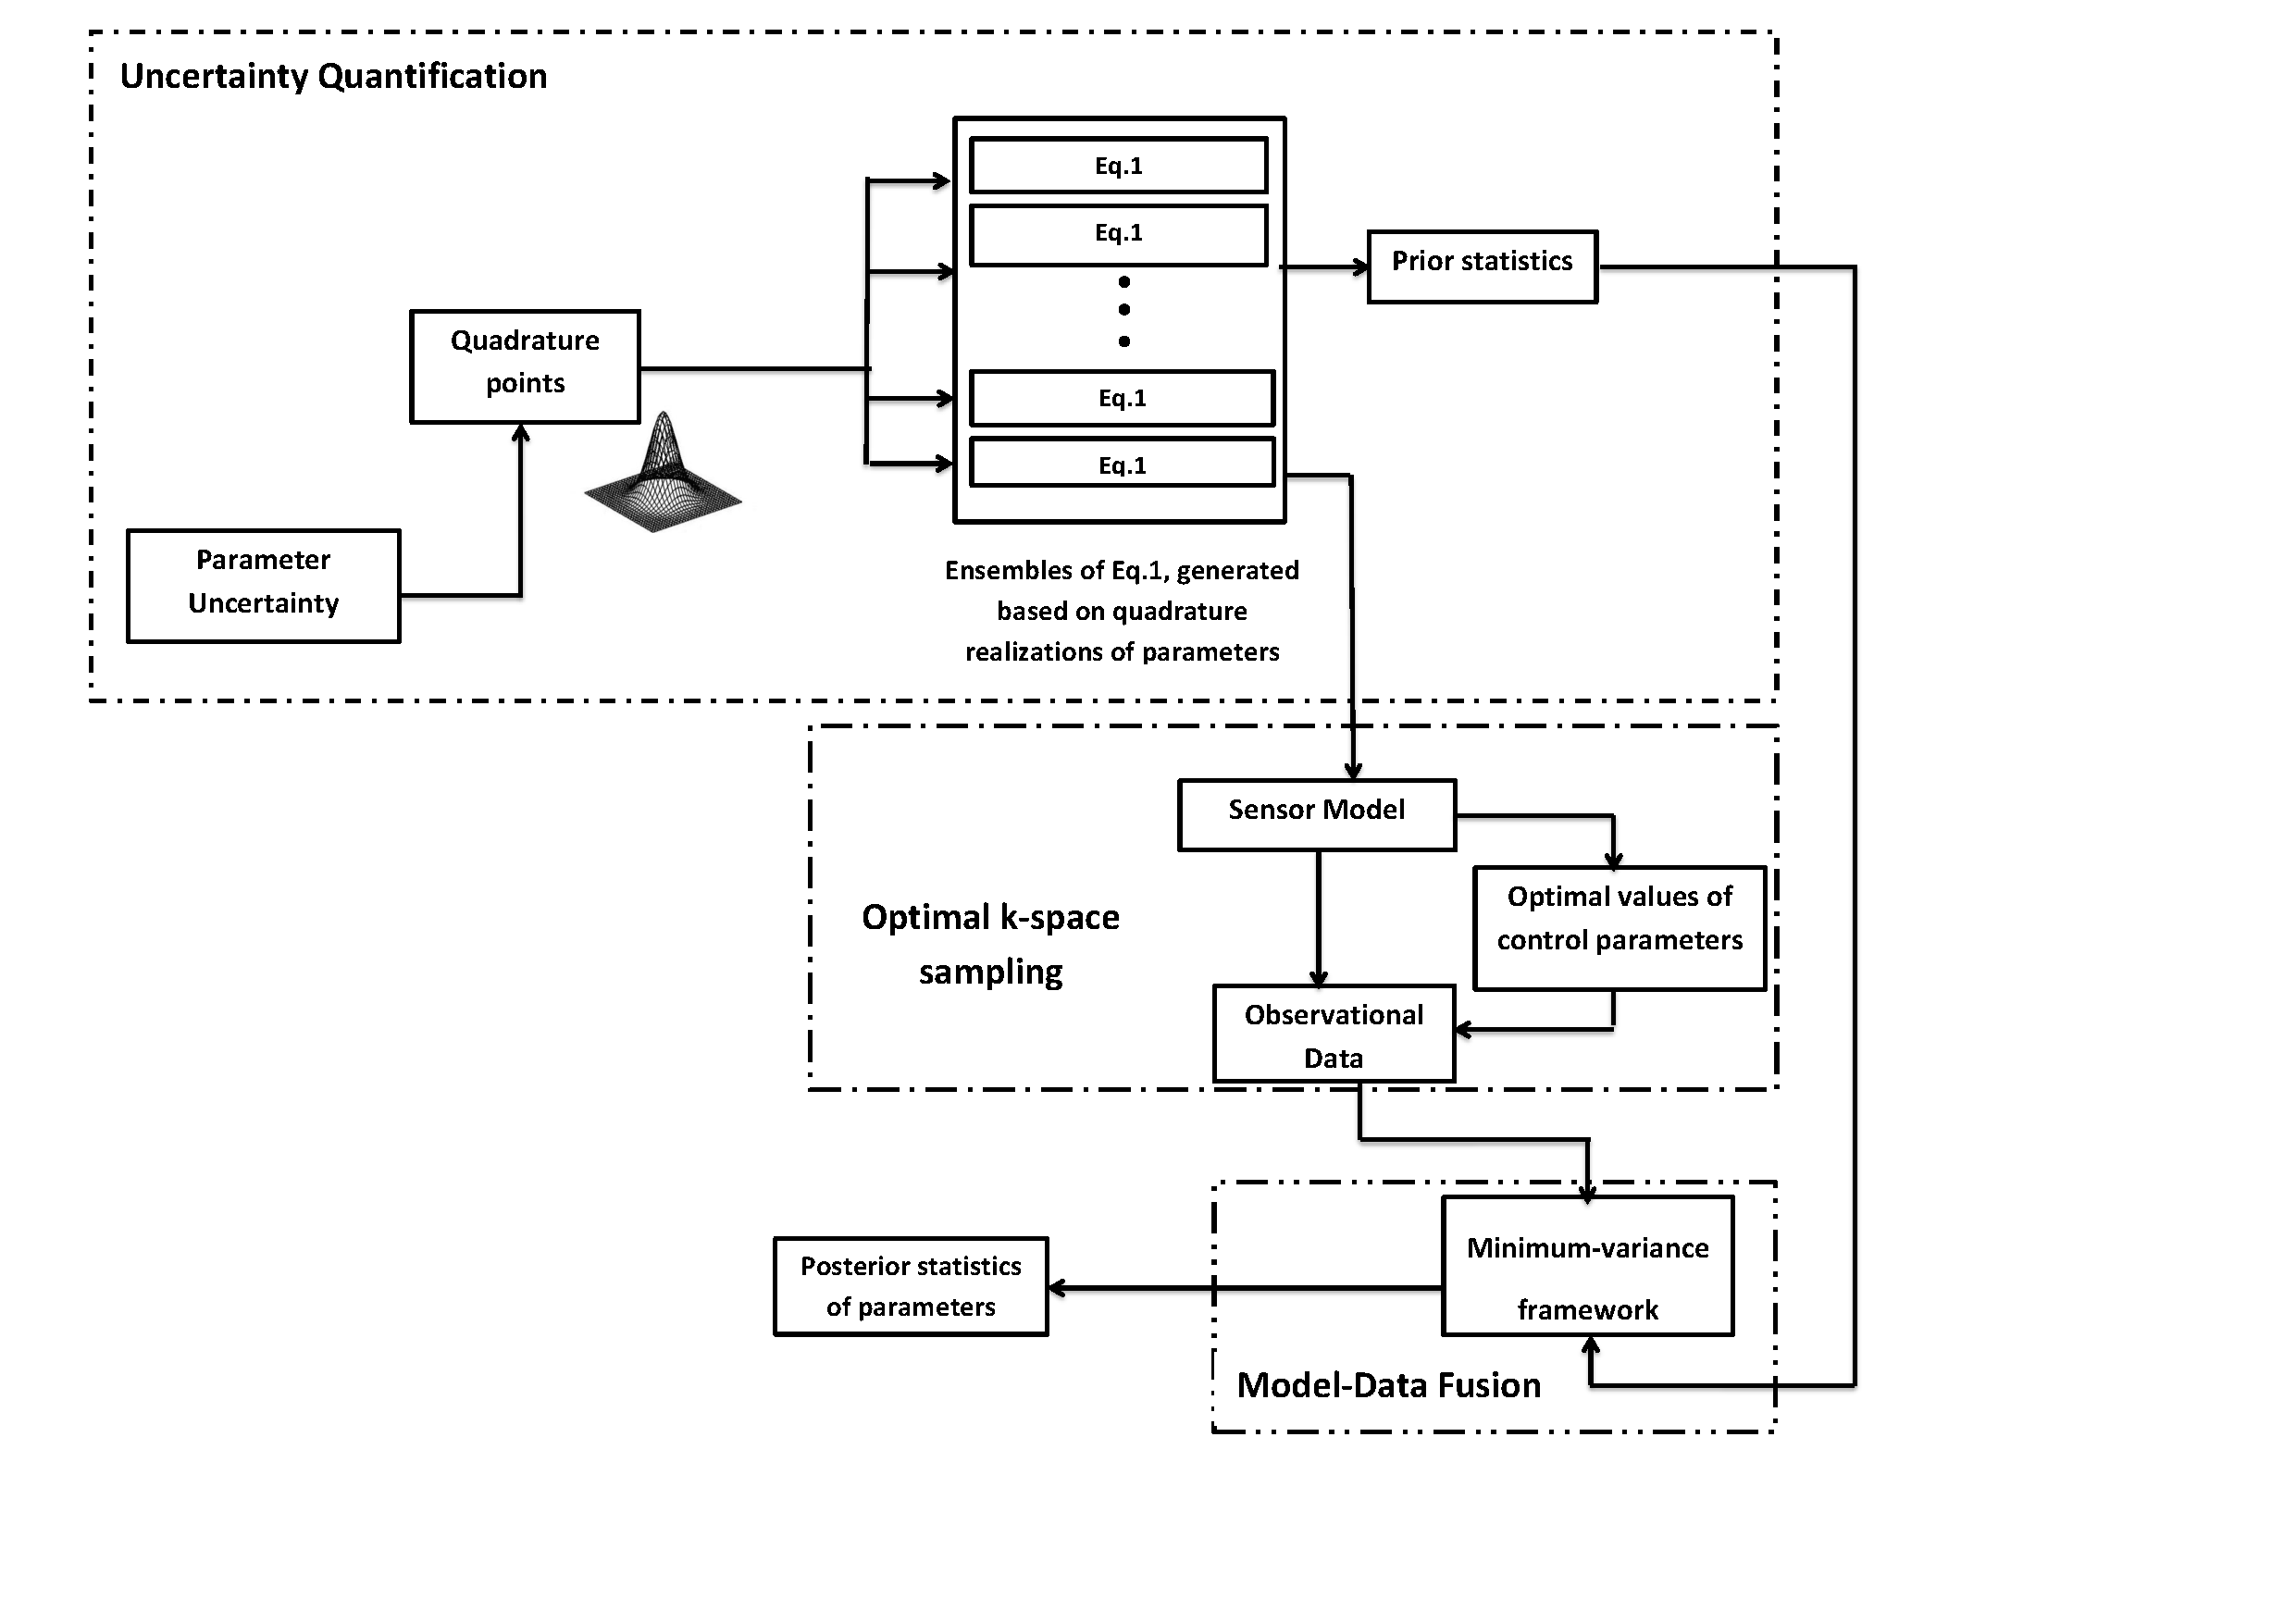
\includegraphics[trim = 1.5cm 3cm 8cm 0.5cm, clip,width=5in,height=4.5in]{\picdir/flowchart.pdf}
\caption{Schematic view of the estimation process}
\end{figure}

\section{WIP - T1, T2, M0 Reconstruction}
\paragraph{Given}
the image space date for  multiple  acquistion parameters 
$\{ M_{TD}(\kk_1),M_{TD}(\kk_2), M_{TD}(\kk_2),... \}$,  \\
 $\kk_i=\{T_{R_i},T_{D_i},\theta_i,T_{E_i},\alpha_i\}$ 
{\color{red}(@kenphwang 2 delay times and 4 echoes correct?)},

The reconstruction algorithms for T1, T2, M0 is as follows:
\begin{itemize}
\item {\color{red}(@kenphwang can we get the current code for this recon.)}
\item {\color{red}(@kenphwang Can  you provide an example data set ? is this real/imaginary data? or magnitude only? is $\alpha$, $\theta$ fixed?)}
\item 
\end{itemize}


%\begin{figure}[htb!]
%\begin{tabular}{ccc}
%\hspace{-0.25in}\subfigure{\includegraphics[width=2.5in]{pics/t2.eps}}&
%\hspace{-0.25in}\subfigure{\includegraphics[width=2.5in]{pics/t2meas.eps}}&
%\hspace{-0.25in}\subfigure{\includegraphics[width=2.5in]{pics/err2.eps}}
%\end{tabular}
%\caption{Temperature map over slice 2 a) Reconstructed temperature, b) observed temperature, c) the error between the reconstruction and measurement.}\label{t2}
%\end{figure}
% % t2 Fig
 


%%%%%%%%%%%%%%%%%%%%%%%%%%%%%%%%%%%%%%%%%%%%%%%%%%%%%%%%%%%%%%%%
\section{ WIP - Physics Model}\label{PhysicsModel}
%%%%%%%%%%%%%%%%%%%%%%%%%%%%%%%%%%%%%%%%%%%%%%%%%%%%%%%%%%%%%%%%
The steady-state magnetization $M_{TD}$ at a specific delay time $T_D$ can be found as a function of flip angle $\theta$, repetition time $T_R$, excitation pulse $\alpha$, and relaxation time  $T_1$:
\[
  M_{TD}  =  M_0\frac{1-(1-\cos(\theta))e^{-\frac{T_D}{T_1}}-\cos(\theta)e^{-\frac{T_R}{T_1}}}{1-\cos(\theta)e^{-\frac{T_R}{T_1}}\cos(\alpha)}
\]
where, $M_0$ is the unsatuarated magnetization.
%%%%%%%%%%%%%%%%%%%%%%%%%%%%%%%%%%%%%%%%%%%%%%%%%%%%%%%%%%%%%%%%
\section{ WIP - Mathematical Framework}\label{GeneralMathFramework}
%%%%%%%%%%%%%%%%%%%%%%%%%%%%%%%%%%%%%%%%%%%%%%%%%%%%%%%%%%%%%%%%

The underlying philosophy and assumptions within our approach is that the physics 
models are 1st order accurate or within 70-80\% of the needed accuracy and the error is
adequate within the assumed Gaussian noise.
Gaussian distributions provide analytical representations of the random
variables of interest (ie T1, T2) within the Bayesian setting and 
provide a crux for understanding. In particular, we say that a random
variable $\eta$ belongs to a multi-variate normal distribution 
of mean $\mu \in \mathbb{R}^n $ and covariance $\Sigma \in \mathbb{R}^{n \times n}$
\[
     \eta \sim \mathcal{N}(\mu,\Sigma)  
    \Rightarrow
      p(\eta)  = \frac{1}{2 \; \pi \; \det{\Sigma}} \exp\left( - \frac{1}{2} \| \mu - \eta\|^2_{\Sigma}\right)
\]


\begin{enumerate}
  \item Our data acquistion model, $\mathcal{G}(\vec{k},\theta): \mathbb{R}^a
\times \mathbb{R}^m \rightarrow \mathbb{R}^n $,
maps deterministic acquisition
parameters, $\vec{k} \in \mathbb{R}^a$, and uncertain parameters, $\theta \in \mathbb{R}^m$
to observables, $\vec{z} \in \mathbb{R}^n$ ( or $\vec{z} \in \mathbb{C}^n$).
Explicitly, we will assume that the
measurement models are corrupted by zero mean white noise noise of a
\textbf{known} covariance matrix, $\Sigma_z \in \mathbb{R}^{n \times n}$ 
\begin{equation}
\label{sensormodelstructure}
\begin{split}
  \vec{z} & = \mathcal{G}(\vec{k};\theta) + \eta   \qquad   \eta \sim \mathcal{N}(0,\Sigma_z)
      \\
  \vec{k} & =  \text{(TE, TR, etc)}
      \\
  \theta &  =  \text{(T1, T2, etc)}
     \end{split}
\end{equation}
$\eta$ may be interpreted as the measurement noise or the acquisition noise
in the sensor model. For a deterministic measurement model $\mathcal{G}$,
the conditional probablity distribution has an explicit analytical form
and may be written as a  \textbf{known} Gaussian
distribution. 
  \[ 
      p(\vec{z}|\theta)   =  \mathcal{N}(\mathcal{G}(\vec{k};\theta),\Sigma_z)  
  \]
  \item Additional \textbf{known} information is the prior probability
distributions for the model parameters, $p(\theta)$.  For simplicity,
    assume that Prior parameters are Gaussian distributed of 
   \textbf{known} mean, $\hat{\theta}$ and covariance, $\Sigma_\theta$
   \[
      \theta \sim \mathcal{N} (\hat{\theta}, \Sigma_\theta)
   \]
  \item Bayes theorem is fundamental to the approach.
The probability of the measurements $p(z)$ must be interprited in terms of the
known information. The probability of the measurements may be derived from
the marginalization of the joint probability and has the interpretation as
the projection of the joint probability onto the measurement axis.
\[
  p(z) = \int_\theta p(\theta,z)  \; d\theta 
       = \int_\theta p(z|\theta) \; p(\theta)\; d\theta 
\]
  \item  The concept of informational entropy~\cite{Madankan15}, $H(Z)$,
provides a mathematically rigorous framework to look for measurement acquisition
parameters, $\vec{k}$, with the high information content of the reconstruction.
Given a probability space 
$(\Omega, \mathcal{F},p)$ (probability maps from the
sigma-algebra of possible events $p:\mathcal{F}\rightarrow [0,1]$
sigma-algebra, $\mathcal{F}$, defined on set of `outcomes' $\Omega$
\cite{durrett2010probability}),
we will define information of an event  as
proportional to the inverse probability.
\[
\text{information} \equiv  \frac{1}{p(z)}
\]
Intuitively, when a low probability event occurs this provides high
information.
The informational entropy is an \textit{average}
of the information content for a sigma algebra of events $\mathcal{F}$
\[
H(Z) = \int_Z  p(z) \ln\frac{1}{p(z)} \; dz
\qquad
  p(z) = \int_\theta p(z|\theta) \; p(\theta)\; d\theta 
\]
Hence this entropy measure is an average of the information content
for a given set of events, $\mathcal{F}$, and is proportional to the
variance or uncertainty in which the set of events occur.
This agrees with thermodynamic entropy;
if the information containing events are completely spread out such as in a
uniform distribution, the entropy is maxmized.
The entropy
is zero for a probability distribution in which
only one event occurs. Zero information is gained when the same event
always occurs ($0 \ln\frac{1}{0} = 0$). 
Intuitively, we want to find acquisition parameters,
$\vec{k}$, for which the measurements are most uncertain
\[
\max_k H(Z)
  \quad \Leftrightarrow \quad
\min_k 
    \int_Z   dz \underbrace{\int_\theta  d\theta \; p(z|\theta) \; p(\theta)}_{p(z)}
                \underbrace{ln \left(\int_\theta  d\theta \; p(z|\theta) \; p(\theta)\right)}_{ln \; p(z)}
\]
Alternatively we may consider this entropy maximization problem as a
sensitivity analysis for the variance of the measurement $Z$, ie . 
$ \max_k H(Z) \approx  \max_k \text{Var}(Z) $
\[ \begin{split}
   \bar{Z} = \mathbb{E}[Z]  & = \int_Z   dz \; z
   \underbrace{\int_\theta  d\theta \; p(z|\theta) \; p(\theta)}_{p(z)}
  \\
   \mathbb{E}[ ( Z - \bar{Z} )^2 ]  & = \int_Z   dz \;(z - \bar{Z})^2 
   \underbrace{\int_\theta  d\theta \; p(z|\theta) \; p(\theta)}_{p(z)}
  \\
   &  \propto
    \int_Z   dz \;(z - \bar{z})^2 \int_\theta  d\theta 
 \exp\left( - \frac{1}{2} \|  z- \mathcal{G}(\vec{k},\theta)  \|^2_{\Sigma_z}\right)
 \exp\left( - \frac{1}{2} \|  \theta - \hat{\theta}  \|^2_{\Sigma_\theta}\right)
 \end{split}
\]
Probilistic integrals may be
computed from uncertainty quantification
techniques~\cite{fahrenholtz2013generalised}.

 

\end{enumerate}

%%%%%%%%%%%%%%%%%%%%%%%%%%%%%%%%%%%%%%%%%%%%%%%%%%%%%%%%%%%%%%%%
\section{WIP - Echo train length }\label{ModelFidelity}
%%%%%%%%%%%%%%%%%%%%%%%%%%%%%%%%%%%%%%%%%%%%%%%%%%%%%%%%%%%%%%%%


% http://mriquestions.com/fse-parameters.html
% http://mriquestions.com/what-is-fsetse.html

In conventional spin-echo imaging, two basic timing parameters are
required, repetition time (TR) and echo time (TE), Figure~\ref{fig:echotrain}(a).
Similar to
fast spin echo (FSE) imaging, 
the acquistion is setup to acquire multiple lines of k-space in a single TR.
In this situation,
TE is replaced by effective echo
time  and addition parameters are needed: 

\begin{itemize}
\item TE$_\text{eff} \equiv$ the time at which the central lines of k-space are being filled.
\item Number of echoes $\equiv$ called echo train length (ETL)
\item Time between echoes $\equiv$ called echo spacing (ESP) 
\end{itemize}



\begin{figure}[h] 
\begin{tabular}{ccc}
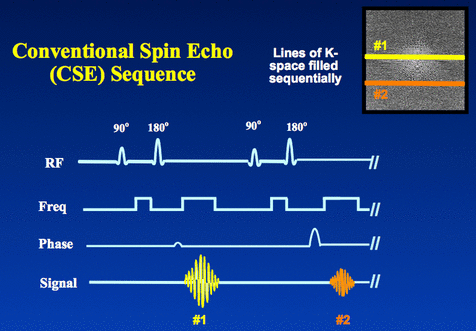
\includegraphics[width=.3\textwidth]{\picdir/7162303.png}
&
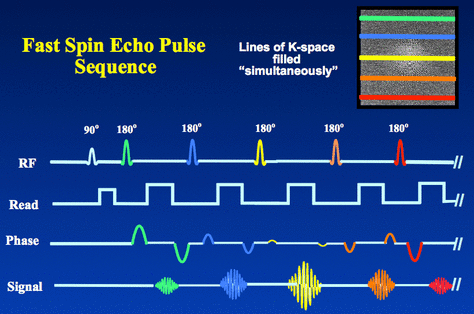
\includegraphics[width=.3\textwidth]{\picdir/5013564.png}
&
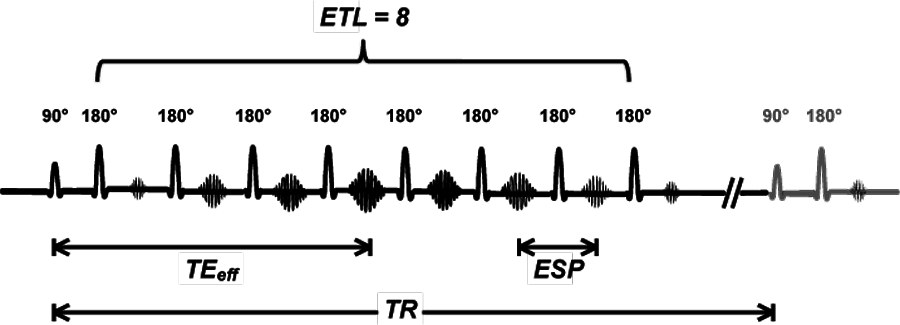
\includegraphics[width=.3\textwidth]{\picdir/3316708_orig.png}
\\
(a) & (b) & (c) \\
\end{tabular}
\caption{ 
(a)
}\label{fig:echotrain}
\end{figure}


{\color{red}
   TODO - need to update signal model for multiple read out lines
}


%%%%%%%%%%%%%%%%%%%%%%%%%%%%%%%%%%%%%%%%%%%%%%%%%%%%%%%%%%%%%%%%
\section{WIP - Inverse Problem Framework}\label{InverseProbFramework}
%%%%%%%%%%%%%%%%%%%%%%%%%%%%%%%%%%%%%%%%%%%%%%%%%%%%%%%%%%%%%%%%
\[
  \vec{z}  = \mathcal{G}(\theta) + \eta   \qquad   \eta \sim \mathcal{N}(0,\Sigma_z)
\]
\[
  p(z|\theta ) = \exp \left( \|\vec{z} -  \mathcal{G}(\theta)\|^2_{\Sigma_z} \right)
\]
\[
               d\left(\vec{z}, \mathcal{G}(\theta^*)\right) = 
   \min_{\theta \in \Omega} d\left(\vec{z}, \mathcal{G}(\theta)\right)
\qquad
\theta = \left(\mu_\text{CSF}, \mu_\text{GM}, \mu_\text{WM}, \mu_\text{Tumor} \right)
\]
%%%%%%%%%%%%%%%%%%%%%%%%%%%%%%%%%%%%%%%%%%%%%%%%%%%%%%%%%%%%%%%%
%%%%%%%%%%%%%%%%%%%%%%%%%%%%%%%%%%%%%%%%%%%%%%%%%%%%%%%%%%%%%%%%
\nocite{*}
\bibliographystyle{apalike}
\bibliography{references}

\appendix
\section{Bayes - An intuitive example}
Bayes theorem is fundamental to the approach and is immediately
follows from the definition of conditional probability
\[
\left.
\begin{split}
p(y|x)  \equiv  \frac{p(x,y)}{p(x)}  \\
p(x|y)  \equiv  \frac{p(x,y)}{p(y)} 
\end{split}
\right\}
\Rightarrow
p(y|x) p(x) = p(x,y) = p(x|y) p(y)
\Rightarrow
\hspace{-1in}
\begin{split}
p(y|x)  =\frac{ p(x|y) p(y) }{p(x) } \\
p(x|y)  =\frac{ p(y|x) p(x) }{p(y) } \\
\end{split}
\]

As a concrete example, consider the explicit two dimensional joint Gaussian
distribution as a medium for understanding. Here we have two random
variables $\mathbf{x}_1$ and $\mathbf{x}_2$ defined on the same probability
space, $\Omega$.
\[
\mathbf{x}_i: \Omega \rightarrow \mathbb{R}
\qquad
P\left( \left\{ \omega: 
\mathbf{x}_i (\omega) \in A
 \right\}\right)
=
\int_A p(\eta_i) d\eta_i
\]
Intuitively, if we are \textbf{given} the joint distribution,
$p(\eta_1,\eta_2)$, knowledge of the realization of one particular random
variable provides information on the realization of the second random
variable.
\[
      p(\eta_1,\eta_2)  = \frac{1}{2 \; \pi \; \sqrt{\det{\Sigma}}}
\exp\left( \frac{1}{2}
\begin{bmatrix}
\eta_1 - \mu_1 \\
\eta_2 - \mu_2 \\
\end{bmatrix}^\top
\underbrace{
\begin{bmatrix}
       \sigma_1^2        & r_{12} \sigma_1 \sigma_2 \\
r_{12} \sigma_1 \sigma_2 &          \sigma_2^2 \\
\end{bmatrix}
}_{\equiv \Sigma}
\begin{bmatrix}
\eta_1 - \mu_1 \\
\eta_2 - \mu_2 \\
\end{bmatrix}
\right)
\]

See \cite{maybeck1979stochastic} (Sec 3.10), characteristic functions 
are used to show that individual marginal
densities of joint  Gaussian random variable is also Gaussian.
\[
p(\eta_1) = 
\int_{\eta_2}
      p(\eta_1,\eta_2)
\;d\eta_2
 = \frac{1}{ \sqrt{2 \; \pi \; \sigma_2^2}} \exp\left( - \frac{(\eta_1 -
\mu_1)^2}{2 \sigma_1^2} \right)
\]

\[
p(\eta_2) = 
\int_{\eta_1}
      p(\eta_2,\eta_1)
\;d\eta_1
 = \frac{1}{ \sqrt{2 \; \pi \; \sigma_1^2}} \exp\left( - \frac{(\eta_2 -
\mu_2)^2}{2 \sigma_2^2} \right)
\]

Conditional probablity is \textit{defined} through the algegraic
reduction of the ratio of the joint and the marginal densities
\[
p(\eta_1|\eta_2) =  \frac{p(\eta_1,\eta_2)  }{p(\eta_2) }
 = \frac{1}{ \sqrt{2 \; \pi \; \sigma_{1|2}^2}}
    \exp\left( - \frac{(\eta_1 - \mu_{1|2})^2}{2 \sigma_{1|2}^2} \right)
 = 
\frac{p(\eta_1)}{p(\eta_2)}
   \frac{1}{ \sqrt{2 \; \pi \; \sigma_{2|1}^2}}
    \exp\left( - \frac{(\eta_2 - \mu_{2|1})^2}{2 \sigma_{2|1}^2} \right)
\]
\[
\mu_{1|2} =  \mu_1 - 
       \frac{r_{12} \sigma_1 \sigma_2 }{\sigma_2^2}
       (\eta_2 - \mu_2)
\qquad
\sigma_{1|2} = 
\sigma_1^2  - 
       \frac{(r_{12} \sigma_1 \sigma_2 )^2}{\sigma_2^2}
\]
\[
\mu_{2|1} =  \mu_2 - 
       \frac{r_{12} \sigma_1 \sigma_2 }{\sigma_1^2}
       (\eta_1 - \mu_1)
\qquad
\sigma_{2|1} = 
\sigma_2^2  - 
       \frac{(r_{12} \sigma_1 \sigma_2 )^2}{\sigma_1^2}
\]

\end{document}
